\documentclass{beamer}
\usepackage{graphicx}
\usepackage{paralist}
\usepackage{outlines}

\title{How Digital Cameras Work}
\author{Mendocino College - Digital Image Manipulation with Photoshop}
\titlegraphic{\vspace{-10mm}
\includegraphics[width = .9\textwidth]{images/photoshop.jpg}} 
\date{\vspace{-5em}} 


\mode <presentation>
\usetheme{Warsaw}
\usecolortheme{default}

\setbeamerfont{footline}{size=\fontsize{5}{8}\selectfont}

\definecolor{darkred}{rgb}{20,0,0}
\definecolor{darkgreen}{RGB}{40,110,20}
\definecolor{darkpurple}{RGB}{30,0,30}
\definecolor{chardonnay}{RGB}{255, 255, 204}

\setbeamercolor*{palette primary}{fg=white, bg=darkgreen}

\setbeamersize{text margin left=0pt, text margin right=0pt}


\begin{document}
	{
		\setbeamertemplate{footline}{} 
		\setbeamertemplate{headline}{} 
		\begin{frame}
			\vspace{-35pt}
			\maketitle
		\end{frame}
	}
		
\section{How the Human Eye Works}

\subsection{How the Human Eye Works}		

\begin{frame}
	\frametitle{How the Human Eye Works}
	\begin{outline}
		\1 First, light passes through the cornea (the clear front layer of the eye). 
		\2 The cornea is shaped like a dome and bends light to help the eye focus.
		\1 Some of this light enters the eye through an opening called the pupil (PYOO-pul). 
		\2 The iris (the colored part of the eye) controls how much light the pupil lets in.
		\1 Light passes through the lens (a clear inner part of the eye). 
		\2 The lens works together with the cornea to focus light correctly on the retina.
		\1 When light hits the retina (a light-sensitive layer of tissue at the back of the eye), special cells called \2 photoreceptors turn the light into electrical signals.
		\1 These electrical signals travel from the retina through the optic nerve to the brain. 
		\2 Then the brain turns the signals into the images you see.
	\end{outline}
\end{frame}

\begin{frame}
	\frametitle{How the Human Eye Works Example}
	\begin{center}
		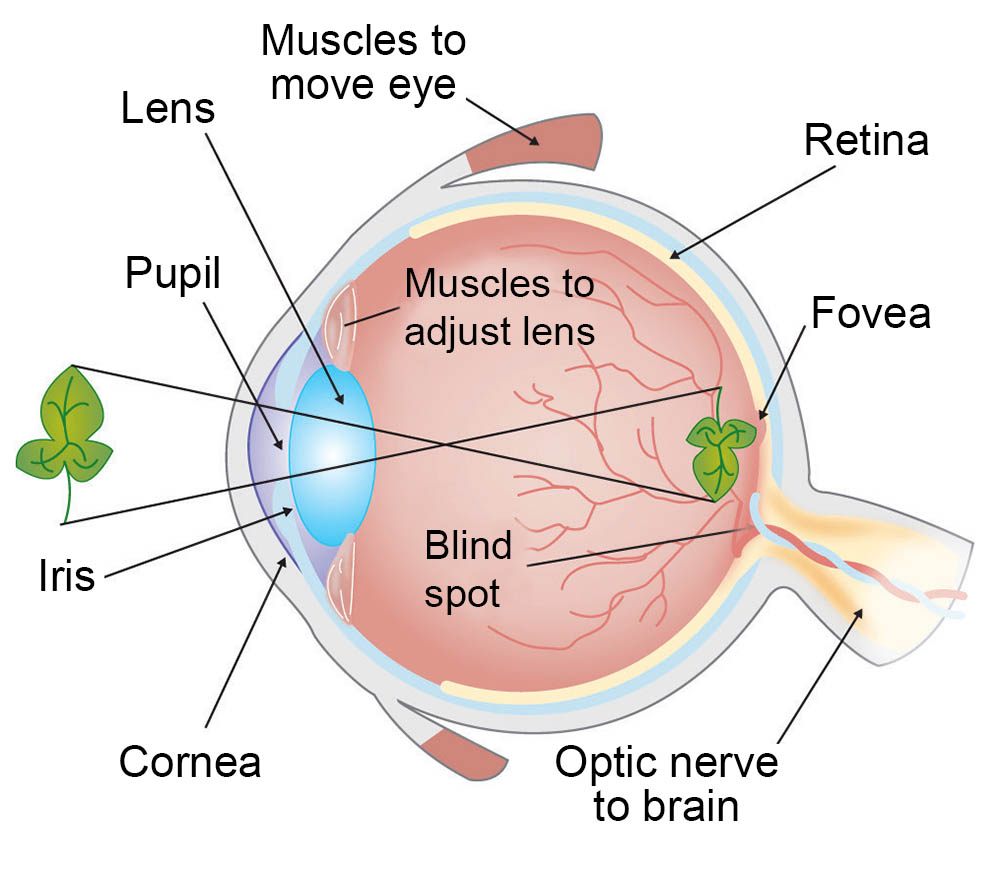
\includegraphics[width=0.8\textwidth]{images/eye-anatomy-1000.jpg}
	\end{center}
\end{frame}


\subsection{The Retina and Photoreceptors}		

\begin{frame}
	\frametitle{The Retina and Photoreceptors}
	\begin{outline}
		\1 The retina also contains the nerves that tell the brain what the photoreceptors are "seeing."
		\1 There are two types of photoreceptors involved in sight: rods and cones.
		\1 Rods work at very low levels of light. 
		\2 We use these for night vision because only a few bits of light (photons) can activate a rod. 
		\2 Rods don't help with color vision, which is why at night, we see everything in a gray scale. 
		\2 The human eye has over 100 million rod cells.
		\1 Cones require a lot more light and they are used to see color. 
		\2 We have three types of cones: blue, green, and red. 
		\2 The human eye only has about 6 million cones.
		\2 Many of these are packed into the fovea, a small pit in the back of the eye that helps with the sharpness or detail of images.
	\end{outline}
\end{frame}

\begin{frame}
	\frametitle{The Retina and photoreceptors Example}
	\begin{center}
		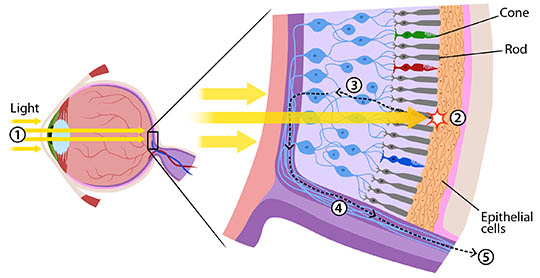
\includegraphics[width=1.0\textwidth]{images/Light-Through-The-Eye.jpg}
	\end{center}
\end{frame}

\subsection{Resources}		
\begin{frame}
	\frametitle{Additional Resources for How Eyes Work}
	\begin{outline}
		\1 How the Eyes Work
		\2 National Eye Institute
		\2 https://www.nei.nih.gov/learn-about-eye-health/healthy-vision/how-eyes-work
		\1 Seeing Color 
		\2 Arizona State University
		\2 https://askabiologist.asu.edu/rods-and-cones
		\1 Vision for Photography
		\2 Ron Dexter
		\2 https://rondexter.com/professional/operation/ vision\_for\_photography.htm
	\end{outline}
\end{frame}

\section{How Film Cameras Work}

\subsection{How Film Cameras Work}		

\begin{frame}
	\frametitle{How Film Cameras Work}
	\begin{outline}
		\1 Before digital cameras came along, photography involved capturing light rays on silver-based film.
		\1 Light enters the front of the camera through the aperture and lens, then hits a piece of film. 
		\1 Film is very sensitive to light: 
		\2 only a tiny amount of light energy is needed to make a photograph and too much light will destroy it. 
		\1 To produce a perfect photo, you have to let exactly the right amount of light hit the film, which is called the exposure. 
		\1 The exposure depends on two factors: 
		\2 How long the shutter is open, measured in seconds (anywhere from 1/10,000 to 30 seconds)
		\1 How wide the Aperture is open, measured in units called f-stops, such as f/4 and f/8. 
		\2 Smaller f numbers (such as 1) means larger apertures, so more light gets in; 
		\2 Higher f numbers (such as 32) means smaller apertures, so less light is let in.
	\end{outline}
\end{frame}

\subsection{Camera Example}		
\begin{frame}
	\frametitle{How Film Cameras Work Example}
	\begin{center}
		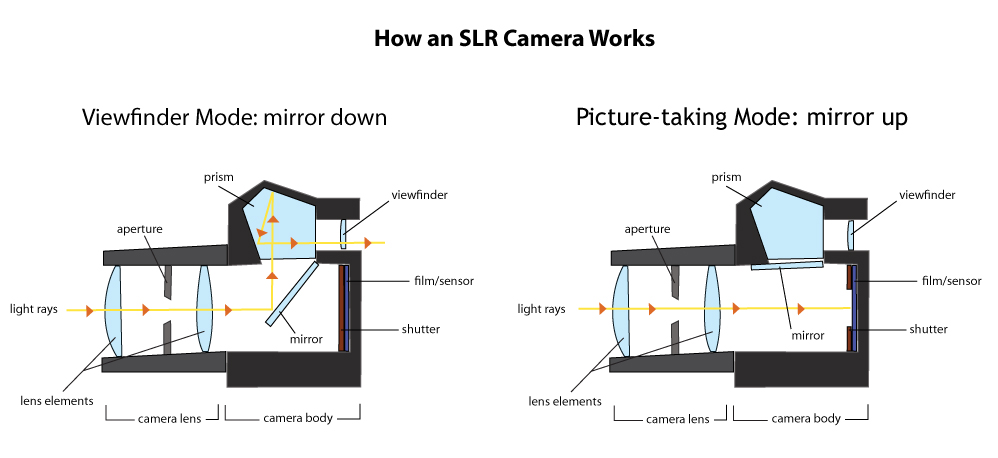
\includegraphics[width=1.10\textwidth]{images/How Camera Works.jpg}
	\end{center}
\end{frame}

\subsection{Lenses}		

\begin{frame}
	\frametitle{Lenses in the Lens}
	\begin{outline}
		\1 A camera lens is actually several lenses combined into one unit. 
		\2 A single converging lens could form a real image on the film, but it would be warped by a number of aberrations.
		\1 One of the most significant warping factors is that different colors of light bend differently when moving through a lens. 
		\2 This chromatic aberration essentially produces an image where the colors are not lined up correctly.
		\1 Cameras compensate for this using several lenses made of different materials. 
		\2 The lenses each handle colors differently, and when you combine them in a certain way, the colors are realigned.
		\1 A standard 50 mm lens doesn't significantly shrink or magnify the image.
	\end{outline}
\end{frame}

\subsection{Lens Example}		
\begin{frame}
	\frametitle{Lens Example}
	\begin{center}
		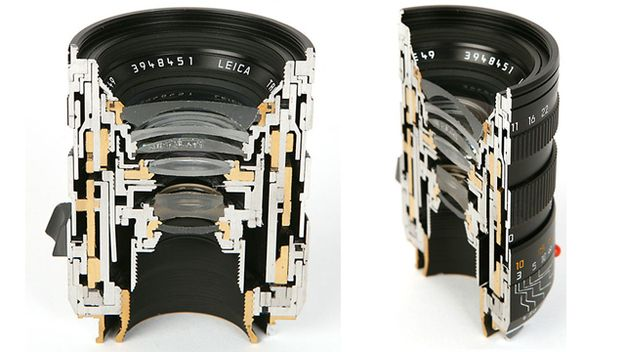
\includegraphics[width=1.0\textwidth]{images/a1e146ea393f65c4858f052816cf9d1d.jpg}
	\end{center}
\end{frame}
	
\begin{frame}
	\frametitle{Additional Resources for How Film Cameras Work}
	\begin{outline}
		\1 35mm Film cameras
		\2  By:  Chris Woodford
		\2 https://www.explainthatstuff.com/how-film-cameras-work.html
		\1 How Cameras Work
		\2  By:  Tom Harris
		\2 https://electronics.howstuffworks.com/camera.htm
	\end{outline}
\end{frame}

		
\section{How Digital Cameras Work}

\subsection{How Digital Cameras Work}		

	\begin{frame}
		\frametitle{How Digital Cameras Work}
		\begin{outline}
			\1 Instead of film, a digital camera has a sensor that converts light into electrical charges.
			\1 The image sensor employed by most digital cameras is a charge coupled device (CCD). 
			\2 Some cameras use complementary metal oxide semiconductor (CMOS) technology instead. 
			\2 Both CCD and CMOS image sensors convert light into electrons.
			\1 Once the sensor converts the light into electrons, it reads the value (accumulated charge) of each cell in the image. 
			\1 Each photosite is colorblind. It only keeps track of the total intensity of the light that strikes its surface. 
			\2 In order to get a full color image, most sensors use filtering to look at the light in its three primary colors. 
			\2 Once the camera records all three colors, it combines them to create the full spectrum.
		\end{outline}
	\end{frame}


\subsection{Example}		
	\begin{frame}
		\frametitle{How Digital Cameras Work Example}
		\begin{center}
			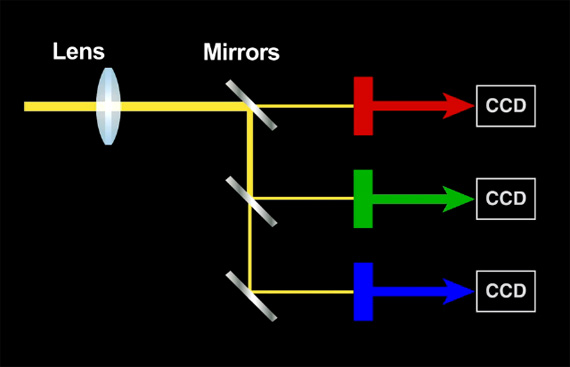
\includegraphics[width=1.0\textwidth]{images/digital-camera-work.jpg}
		\end{center}
	\end{frame}

\subsection{Exposure and Focus}		
\begin{frame}
	\frametitle{Exposure and Focus}
	\begin{outline}
	\1 Just as with film, a digital camera has to control the amount of light that reaches the sensor. 
	\2 The two components it uses to do this, the aperture and shutter speed, are also present on conventional cameras.
	\1 The camera also has to adjust the lenses to control how the light is focused on the sensor. 
	\1 The focal length, however, is one important difference between the lens of a digital camera and the lens of a 35mm camera. 
	\2 The focal length is the distance between the lens and the surface of the sensor. 
	\2 Sensors are in general smaller than a piece of 35mm film. 
	\2 In order to project the image onto a smaller sensor, the focal length is shortened by the same proportion. 
\end{outline}
\end{frame}

\subsection{Resources}		
	\begin{frame}
		\frametitle{Additional Resources for the How Digital Cameras Work}
		\begin{outline}
			\1 DIGITAL CAMERA SENSOR SIZES
			\2  By:  Cambridge in Colour
			\2 https://www.cambridgeincolour.com/tutorials/digital-camera-sensor-size.htm
			\1 Digital cameras
			\2  By:  Chris Woodford
			\2 https://www.explainthatstuff.com/digitalcameras.html
		\end{outline}
	\end{frame}

\section{Comparing Eyes to Cameras}		
\subsection{Comparing Eyes to Cameras}		

\begin{frame}
	\frametitle{Comparing Eyes to Cameras}
	\begin{outline}
		\1 The focal length of the eye is about 17 mm (2/3"). 
		\1 We see almost 180 degrees wide, 120 degrees high
		\1 If you think of the eye as a camera, then: 
		\2 The Cornea would be the Lens.
		\2 The Iris would be the Aperture.  
		\2 The Retina would be the Film.
	\end{outline}
\end{frame}
	
\end{document}